\documentclass{ximera}

\input{../preamble.tex}

\outcome{Understand the properties of trigonometric functions.}
\outcome{Evaluate expressions and solve equations involving
          trigonometric functions and inverse trigonometric functions.}
\outcome{Evaluate limits involving trigonometric functions.}

\title{5.1 - Trigonometric functions}

\begin{document}
\begin{abstract}
  We introduce trigonometric functions.
\end{abstract}
\maketitle

\section{Angles}
An angle is the amount of rotation between two vectors--and initial side and a terminal side--sharing an endpoint. An angle in \dfn{standard position} is assumed to have initial side on the positive $x$-axis, with positive angles rotating counterclockwise about the origin and negative angles rotating clockwise about the origin. A positive angle $\theta$ in standard position is shown below; when the terminal side is length $1$, angles trace out the \dfn{unit circle}, which is a circle centered at $(0,0)$ with radius $1$.

\begin{image}[2in]
\begin{tikzpicture}
	\begin{axis}[
            xmin=-1.1,xmax=1.1,ymin=-1.1,ymax=1.1,
            axis lines=center,
            width=4in,
            xtick={-1,1},
            ytick={-1,1},
            clip=false,
            unit vector ratio*=1 1 1,
            xlabel=$x$, ylabel=$y$,
            every axis y label/.style={at=(current axis.above origin),anchor=south},
            every axis x label/.style={at=(current axis.right of origin),anchor=west},
          ]        
          \addplot [dashed, smooth, domain=(0:360)] ({cos(x)},{sin(x)}); %% unit circle
          \addplot [thick, penColor] plot coordinates {(0,0) (.766,.643)}; %% 40 degrees
          \addplot [thick, penColor2] plotcoordinates {(0,0) (1,0)};
          \addplot [textColor,smooth, domain=(0:40)] ({.15*cos(x)},{.15*sin(x)});
          \node at (axis cs:.15,.07) [anchor=west] {$\theta$};
          \node[textColor, rotate=40] at (axis cs:.35,.38) {terminal side};
          \node[textColor] at (axis cs:.5,-.07) {initial side};
%          \draw (.766, .643) node[circle,fill,inner sep=1pt, label=above:$(\cos(\theta), \sin(\theta))$](a){};
        \end{axis}
\end{tikzpicture}
\end{image}

Angles can be measured in degrees or in radians. \dfn{Degrees} simply divide the full circle into $360$ equal pizza slices, so $360^{\circ}$ is a full rotation, $180^{\circ}$ is a half rotation, and $90^{\circ}$ is a right angle in standard position. Mathematicians typically prefer to use radians, however. The \dfn{radian} measure of an angle is exactly the length of the intercepted edge of the unit circle it traces out. Since the unit circle has circumference $2\pi r=2\pi(1)=2\pi$, that means $360^{\circ}$ and $2\pi$ radians are equivalent, as are $90^{\circ}$ and $\pi/2$ radians.  The $16$ standard angles of the unit circle are shown below, in both degrees and radians.

\begin{image}
\begin{tikzpicture}[scale=5,cap=round,>=latex]
        % draw the coordinates
        \draw[->] (-1.5cm,0cm) -- (1.5cm,0cm) node[right,fill=white] {$x$};
        \draw[->] (0cm,-1.5cm) -- (0cm,1.5cm) node[above,fill=white] {$y$};

        % draw the unit circle
        \draw[thick] (0cm,0cm) circle(1cm);

        \foreach \x in {0,30,...,360} {
                % lines from center to point
                \draw[gray] (0cm,0cm) -- (\x:1cm);
                % dots at each point
                \filldraw[black] (\x:1cm) circle(0.4pt);
                % draw each angle in degrees
                \draw (\x:0.6cm) node[fill=white] {$\x^\circ$};
        }
             \foreach \x in {0,45,...,360} {
                % lines from center to point
                \draw[gray] (0cm,0cm) -- (\x:1cm);
                % dots at each point
                \filldraw[black] (\x:1cm) circle(0.4pt);
                % draw each angle in degrees
                \draw (\x:0.6cm) node[fill=white] {$\x^\circ$};
        }

        % draw each angle in radians
        \foreach \x/\xtext in {
            30/\frac{\pi}{6},
            45/\frac{\pi}{4},
            60/\frac{\pi}{3},
            90/\frac{\pi}{2},
            120/\frac{2\pi}{3},
            135/\frac{3\pi}{4},
            150/\frac{5\pi}{6},
            180/\pi,
            210/\frac{7\pi}{6},
            225/\frac{5\pi}{4},
            240/\frac{4\pi}{3},
            270/\frac{3\pi}{2},
            300/\frac{5\pi}{3},
            315/\frac{7\pi}{4},
            330/\frac{11\pi}{6},
            360/2\pi}
                \draw (\x:0.85cm) node[fill=white] {$\xtext$};

%        \foreach \x/\xtext/\y in {
%            % the coordinates for the first quadrant
%            30/\frac{\sqrt{3}}{2}/\frac{1}{2},
%            45/\frac{\sqrt{2}}{2}/\frac{\sqrt{2}}{2},
%            60/\frac{1}{2}/\frac{\sqrt{3}}{2},
%            % the coordinates for the second quadrant
%            150/-\frac{\sqrt{3}}{2}/\frac{1}{2},
%            135/-\frac{\sqrt{2}}{2}/\frac{\sqrt{2}}{2},
%            120/-\frac{1}{2}/\frac{\sqrt{3}}{2},
%            % the coordinates for the third quadrant
%            210/-\frac{\sqrt{3}}{2}/-\frac{1}{2},
%            225/-\frac{\sqrt{2}}{2}/-\frac{\sqrt{2}}{2},
%            240/-\frac{1}{2}/-\frac{\sqrt{3}}{2},
%            % the coordinates for the fourth quadrant
%            330/\frac{\sqrt{3}}{2}/-\frac{1}{2},
%            315/\frac{\sqrt{2}}{2}/-\frac{\sqrt{2}}{2},
%            300/\frac{1}{2}/-\frac{\sqrt{3}}{2}}
%                \draw (\x:1.25cm) node[fill=white] {$\left(\xtext,\y\right)$};

        % draw the horizontal and vertical coordinates
        % the placement is better this way
        \draw (-1.25cm,0cm) node[above=1pt] {$(-1,0)$}
              (1.25cm,0cm)  node[above=1pt] {$(1,0)$}
              (0cm,-1.25cm) node[fill=white] {$(0,-1)$}
              (0cm,1.25cm)  node[fill=white] {$(0,1)$};
    \end{tikzpicture}
\end{image}
    
\begin{example}
Which of the $16$ standard angles above has the same terminal side as $-\dfrac{\pi}{4}$ radians? 
\\$\answer[given]{\dfrac{7\pi}{4}}$ radians or $\answer[given]{315}$ degrees
\end{example}

\begin{example}
Which of the $16$ standard angles above has the same terminal side as $\dfrac{11\pi}{4}$ radians? 
\begin{explanation}
This angle is greater than a full rotation of $2\pi$. Since $2\pi=8\pi/4$, if we count in steps of $\pi/4$ around the unit circle we pass $8\pi/4$ as we complete a full rotation, and then go $3\pi/4$ more. Thus, we land at
$\answer[given]{\dfrac{3\pi}{4}}$ radians or $\answer[given]{135}$ degrees

\end{explanation}
\end{example}


\subsection{Conversion between degrees and radians}
To convert an angle from degrees to radians, multiply it by the conversion factor $\pi/180^{\circ}$. To convert an angle from radians to degrees, multiply it by its reciprocal $180^{\circ}/\pi$.

\begin{example}

$45^{\circ}=45^{\circ}\cdot\dfrac{\pi}{180^{\circ}}=\frac{\pi}{4}$
\\$18^{\circ}=18^{\circ}\cdot\dfrac{\pi}{180^{\circ}}=\answer[given]{\frac{\pi}{10}}$
\\$\dfrac{2\pi}{3}= \dfrac{2\pi}{3}\cdot\dfrac{180^{\circ}}{\pi}=120^{\circ}$\\
\\$\dfrac{7\pi}{6}= \dfrac{7\pi}{6}\cdot\dfrac{180^{\circ}}{\pi}=\answer[given]{210}^{\circ}$

Notice that angles given in radians often have no units stated, as radians are in the same units as $x$ or $y$.

\end{example}
\section{What are trigonometric functions?}
%
%\begin{definition}
%  A \dfn{trigonometric function} is a function that relates a measure
%  of an angle of a right triangle to a ratio of the triangle's sides.
%\end{definition}


The basic trigonometric functions are cosine and sine. 

\begin{definition}
The \dfn{cosine} of angle $\theta$, written $\cos(\theta)$, is the $x$ value of the intersection of the terminal side of $\theta$ and the unit circle. 
\\\\The \dfn{sine} of angle $\theta$, written $\sin(\theta)$, is the $y$ value of the intersection of the terminal side of $\theta$ and the unit circle. That is, the terminal side of angle $\theta$ intersects the unit circle at the point $(x,y)=(\cos(\theta),\sin(\theta))$.
\end{definition}

For example, the angle $\theta=\pi/2$ intersects the unit circle at the point $(0,1)$, so $\cos(\pi/2)=0$ and $\sin(\pi/2)=1$. We can use the Pythagorean Theorem to compute the $x$ and $y$ values of all $16$ standard points on the unit circle:

\begin{image}
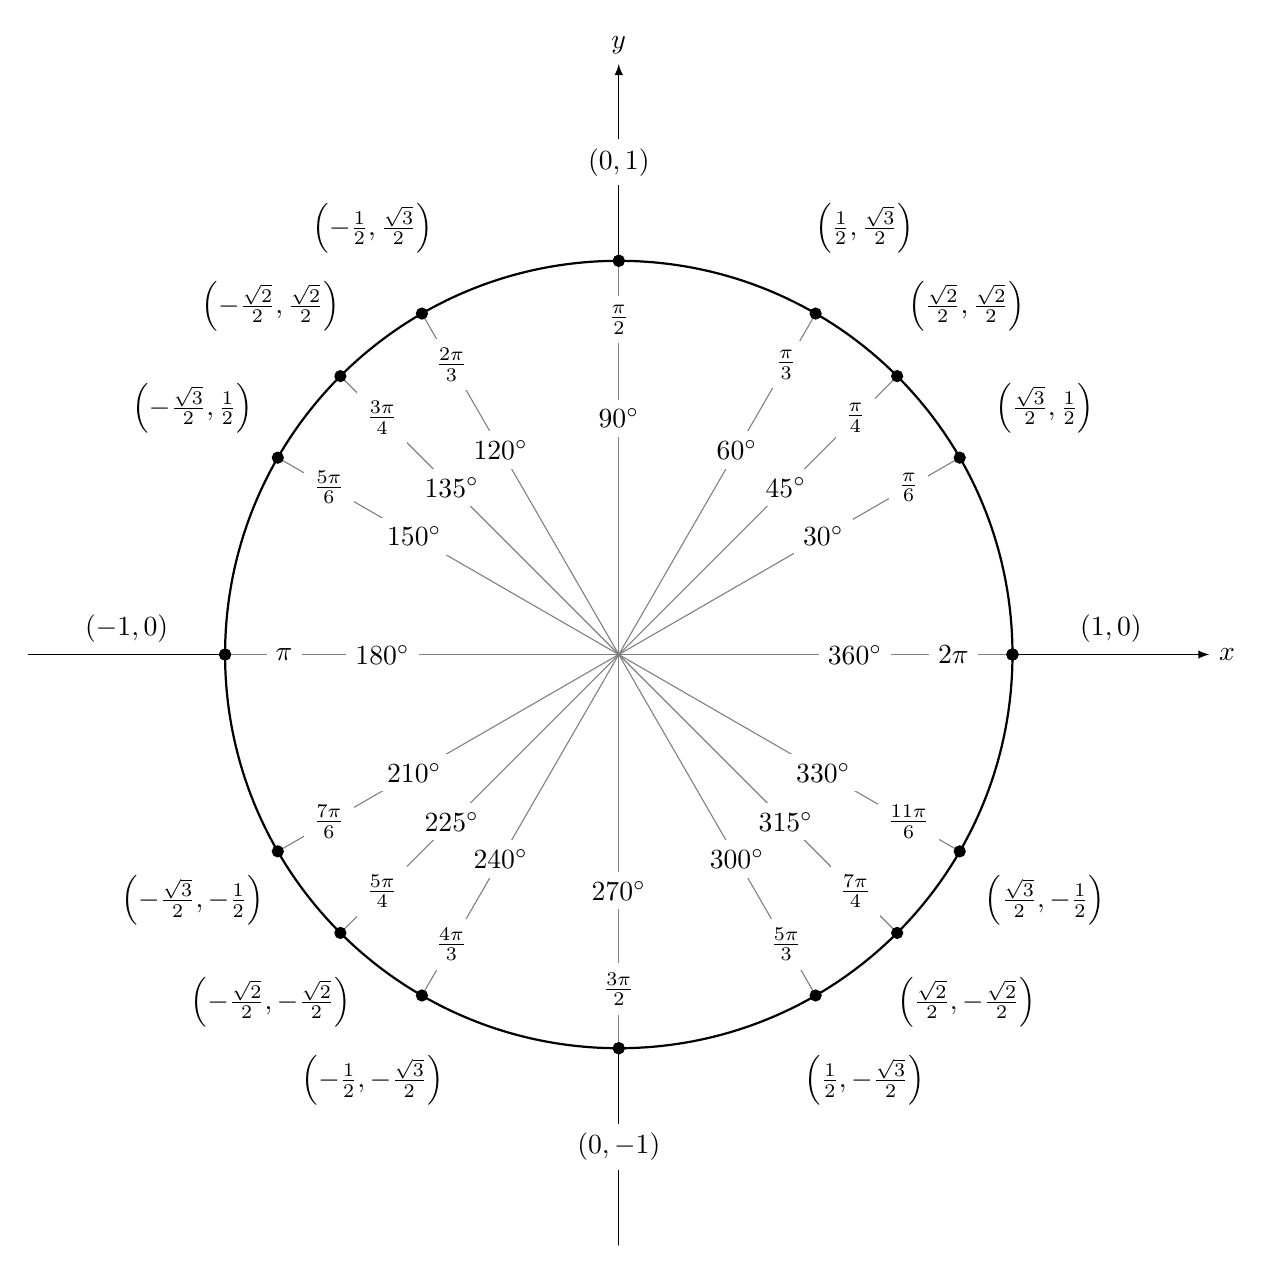
\begin{tikzpicture}[scale=5,cap=round,>=latex]
        % draw the coordinates
        \draw[->] (-1.5cm,0cm) -- (1.5cm,0cm) node[right,fill=white] {$x$};
        \draw[->] (0cm,-1.5cm) -- (0cm,1.5cm) node[above,fill=white] {$y$};

        % draw the unit circle
        \draw[thick] (0cm,0cm) circle(1cm);

        \foreach \x in {0,30,...,360} {
                % lines from center to point
                \draw[gray] (0cm,0cm) -- (\x:1cm);
                % dots at each point
                \filldraw[black] (\x:1cm) circle(0.4pt);
                % draw each angle in degrees
                \draw (\x:0.6cm) node[fill=white] {$\x^\circ$};
        }
             \foreach \x in {0,45,...,360} {
                % lines from center to point
                \draw[gray] (0cm,0cm) -- (\x:1cm);
                % dots at each point
                \filldraw[black] (\x:1cm) circle(0.4pt);
                % draw each angle in degrees
                \draw (\x:0.6cm) node[fill=white] {$\x^\circ$};
        }

        % draw each angle in radians
        \foreach \x/\xtext in {
            30/\frac{\pi}{6},
            45/\frac{\pi}{4},
            60/\frac{\pi}{3},
            90/\frac{\pi}{2},
            120/\frac{2\pi}{3},
            135/\frac{3\pi}{4},
            150/\frac{5\pi}{6},
            180/\pi,
            210/\frac{7\pi}{6},
            225/\frac{5\pi}{4},
            240/\frac{4\pi}{3},
            270/\frac{3\pi}{2},
            300/\frac{5\pi}{3},
            315/\frac{7\pi}{4},
            330/\frac{11\pi}{6},
            360/2\pi}
                \draw (\x:0.85cm) node[fill=white] {$\xtext$};

        \foreach \x/\xtext/\y in {
            % the coordinates for the first quadrant
            30/\frac{\sqrt{3}}{2}/\frac{1}{2},
            45/\frac{\sqrt{2}}{2}/\frac{\sqrt{2}}{2},
            60/\frac{1}{2}/\frac{\sqrt{3}}{2},
            % the coordinates for the second quadrant
            150/-\frac{\sqrt{3}}{2}/\frac{1}{2},
            135/-\frac{\sqrt{2}}{2}/\frac{\sqrt{2}}{2},
            120/-\frac{1}{2}/\frac{\sqrt{3}}{2},
            % the coordinates for the third quadrant
            210/-\frac{\sqrt{3}}{2}/-\frac{1}{2},
            225/-\frac{\sqrt{2}}{2}/-\frac{\sqrt{2}}{2},
            240/-\frac{1}{2}/-\frac{\sqrt{3}}{2},
            % the coordinates for the fourth quadrant
            330/\frac{\sqrt{3}}{2}/-\frac{1}{2},
            315/\frac{\sqrt{2}}{2}/-\frac{\sqrt{2}}{2},
            300/\frac{1}{2}/-\frac{\sqrt{3}}{2}}
                \draw (\x:1.25cm) node[fill=white] {$\left(\xtext,\y\right)$};

        % draw the horizontal and vertical coordinates
        % the placement is better this way
        \draw (-1.25cm,0cm) node[above=1pt] {$(-1,0)$}
              (1.25cm,0cm)  node[above=1pt] {$(1,0)$}
              (0cm,-1.25cm) node[fill=white] {$(0,-1)$}
              (0cm,1.25cm)  node[fill=white] {$(0,1)$};
    \end{tikzpicture} \end{image}

\begin{example}
Using the unit circle above, determine the given trigonometric value.
\\$\cos(45^{\circ})=\answer{\sqrt{2}/2}$
\\$\cos(\pi)=\answer{-1}$
\\$\sin(\pi)=\answer{0}$
\\$\sin(7\pi/6)=\answer{-1/2}$
\end{example}

Without access to a unit circle or a calculator, this at first appears to be an astronomical amount of memorization, but the key is to observe a pattern in the coordinates of the points. Notice that all four angles sitting $\pi/6$ (or $30^{\circ}$) from the $x$-axis in any direction all have the same $(x,y)$ coordinates, give or take a few minus signs. This is also true about the four angles that are $\pi/$ (or $45^{\circ}$) from the $x$-axis and all four angles $\pi/3$ (or $60^{\circ}$) from the $x$-axis.

\begin{image}
\begin{tikzpicture}[scale=3,cap=round,>=latex]
        % draw the coordinates
        \draw[->] (-1.5cm,0cm) -- (1.5cm,0cm) node[right,fill=white] {$x$};
        \draw[->] (0cm,-1.5cm) -- (0cm,1.5cm) node[above,fill=white] {$y$};

        % draw the unit circle
        \draw[thick] (0cm,0cm) circle(1cm);

        \foreach \x in {30,150, 210, 330} {
                % lines from center to point
                \draw[gray] (0cm,0cm) -- (\x:1cm);
                % dots at each point
                \filldraw[black] (\x:1cm) circle(0.4pt);
                % draw each angle in degrees
                \draw (\x:0.6cm) node[fill=white] {$\x^\circ$};
        }
        % draw each angle in radians
        \foreach \x/\xtext in {
            30/\frac{\pi}{6},
            150/\frac{5\pi}{6},
            210/\frac{7\pi}{6},
            330/\frac{11\pi}{6}}
                \draw (\x:0.85cm) node[fill=white] {$\xtext$};

        \foreach \x/\xtext/\y in {
            30/\frac{\sqrt{3}}{2}/\frac{1}{2},
            150/-\frac{\sqrt{3}}{2}/\frac{1}{2},
            210/-\frac{\sqrt{3}}{2}/-\frac{1}{2},        
            330/\frac{\sqrt{3}}{2}/-\frac{1}{2}
         }
                \draw (\x:1.25cm) node[fill=white] {$\left(\xtext,\y\right)$};

        % draw the horizontal and vertical coordinates
        % the placement is better this way

    \end{tikzpicture} \end{image}
    
\begin{image}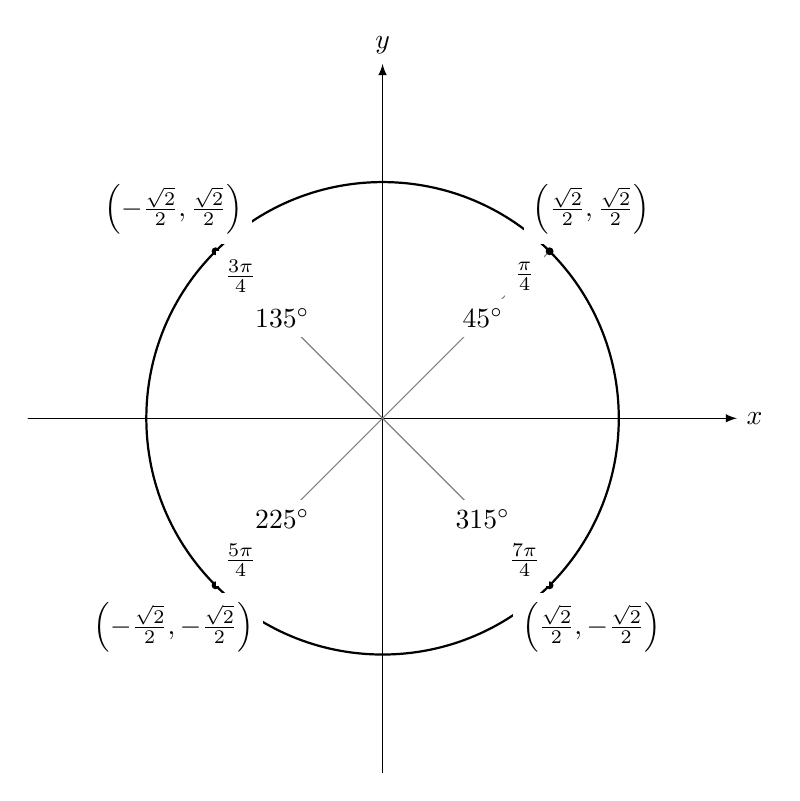
\begin{tikzpicture}[scale=3,cap=round,>=latex]
        % draw the coordinates
        \draw[->] (-1.5cm,0cm) -- (1.5cm,0cm) node[right,fill=white] {$x$};
        \draw[->] (0cm,-1.5cm) -- (0cm,1.5cm) node[above,fill=white] {$y$};

        % draw the unit circle
        \draw[thick] (0cm,0cm) circle(1cm);

        \foreach \x in {45,135,225,315} {
                % lines from center to point
                \draw[gray] (0cm,0cm) -- (\x:1cm);
                % dots at each point
                \filldraw[black] (\x:1cm) circle(0.4pt);
                % draw each angle in degrees
                \draw (\x:0.6cm) node[fill=white] {$\x^\circ$};
        }

        % draw each angle in radians
        \foreach \x/\xtext in {
            45/\frac{\pi}{4},
            135/\frac{3\pi}{4},
            225/\frac{5\pi}{4},
            315/\frac{7\pi}{4}}
                \draw (\x:0.85cm) node[fill=white] {$\xtext$};

        \foreach \x/\xtext/\y in {
            45/\frac{\sqrt{2}}{2}/\frac{\sqrt{2}}{2},
            135/-\frac{\sqrt{2}}{2}/\frac{\sqrt{2}}{2},
            225/-\frac{\sqrt{2}}{2}/-\frac{\sqrt{2}}{2},
            315/\frac{\sqrt{2}}{2}/-\frac{\sqrt{2}}{2}}
                \draw (\x:1.25cm) node[fill=white] {$\left(\xtext,\y\right)$};
    \end{tikzpicture} \end{image}

\begin{image}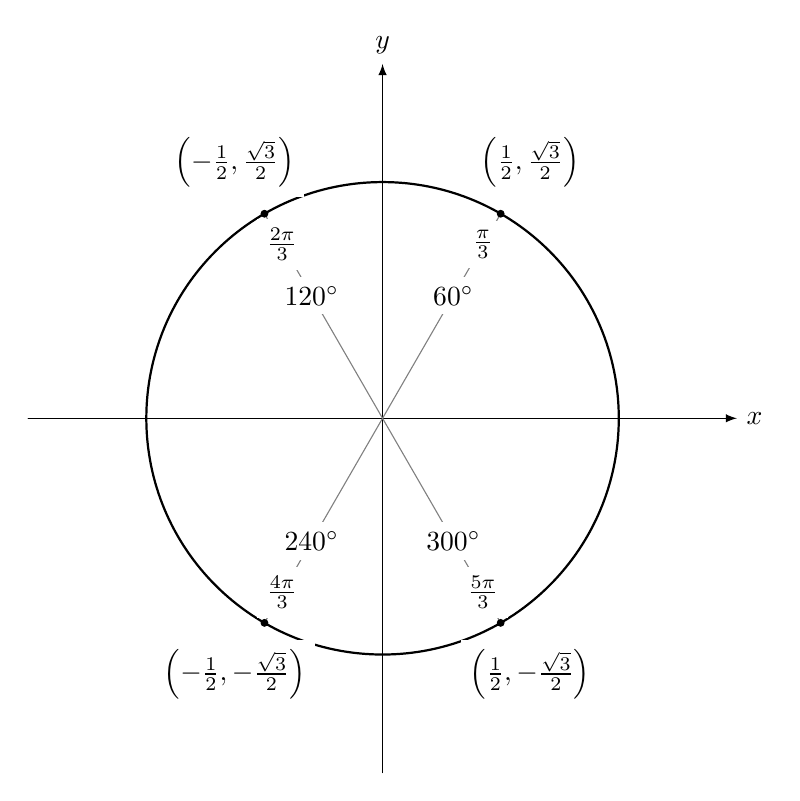
\begin{tikzpicture}[scale=3,cap=round,>=latex]
        % draw the coordinates
        \draw[->] (-1.5cm,0cm) -- (1.5cm,0cm) node[right,fill=white] {$x$};
        \draw[->] (0cm,-1.5cm) -- (0cm,1.5cm) node[above,fill=white] {$y$};

        % draw the unit circle
        \draw[thick] (0cm,0cm) circle(1cm);

        \foreach \x in {60,120,240,300} {
                % lines from center to point
                \draw[gray] (0cm,0cm) -- (\x:1cm);
                % dots at each point
                \filldraw[black] (\x:1cm) circle(0.4pt);
                % draw each angle in degrees
                \draw (\x:0.6cm) node[fill=white] {$\x^\circ$};
        }
        % draw each angle in radians
        \foreach \x/\xtext in {
            60/\frac{\pi}{3},
            120/\frac{2\pi}{3},
            240/\frac{4\pi}{3},
            300/\frac{5\pi}{3}}
                \draw (\x:0.85cm) node[fill=white] {$\xtext$};

        \foreach \x/\xtext/\y in {
            60/\frac{1}{2}/\frac{\sqrt{3}}{2},
            120/-\frac{1}{2}/\frac{\sqrt{3}}{2},
            240/-\frac{1}{2}/-\frac{\sqrt{3}}{2},
            300/\frac{1}{2}/-\frac{\sqrt{3}}{2}}
                \draw (\x:1.25cm) node[fill=white] {$\left(\xtext,\y\right)$};
    \end{tikzpicture} \end{image}
    
Thus we need only memorize the $(x,y)$ coordinates of the angles in the first quadrant. When we are presented with an angle $\theta$, we associate it with one of these three angles (its ``reference angle") to determine the magnitude. Then we use its quadrant to determine the sign.

\begin{example}
Compute $\cos(3\pi/4)$ and $\sin(3\pi/4)$.
\begin{explanation}
We plot the angle $3\pi/4$ and see that it is $45^{\circ}$ from the $x$-axis in the second quadrant. This means that $45^{\circ}$ or $\pi/4$ is its reference angle. Thus the magnitude of its cosine and sine values are the same as those of $\pi/4$, which are both $\sqrt{2}/2$. Since $3\pi/4$ is in the second quadrant, we reason that its cosine ($x$ value) is negative and its sine ($y$ value) is positive. Thus we conclude that $\cos(3\pi/4)=-\sqrt{2}/2$ and $\sin(3\pi/4)=\sqrt{2}/2$.
\end{explanation}
\end{example}    

\begin{definition}[The Other Trig Functions]
For an angle $\theta$ in standard position, we define the following four additional trigonometric functions and their abbreviations:
\\
\\\dfn{tangent:} $\tan(\theta)=\dfrac{\sin(\theta)}{\cos(\theta)}$
\\\dfn{secant:} $\sec(\theta)=\dfrac{1}{\cos(\theta)}$
\\\dfn{cosecant:} $\csc(\theta)=\dfrac{1}{\sin(\theta)}$
\\\dfn{cotangent:} $\cot(\theta)=\dfrac{\cos(\theta)}{\sin(\theta)}$
\end{definition}
    
\begin{example}
Compute the following trig values.
\\$\tan(\pi/4)=\dfrac{\sin(\pi/4)}{\cos(\pi/4)}=\dfrac{\sqrt{2}/2}{\sqrt{2}/2}=1$
\\$\sec(\pi/6)=\dfrac{1}{\cos(\pi/6)}=\dfrac{1}{\answer{\sqrt{3}/2}}=\dfrac{2}{\sqrt{3}}$ or $\dfrac{2\sqrt{3}}{3}$

\end{example}    
    
Notice that while cosine and sine are defined for all possible inputs, whenever we encounter division by zero the other four trig functions will be undefined. For example, quantities like $\tan(\pi/2)$ and $\csc(0)$ are undefined.
    
\section{Triangle Trigonometry}

As an alternative to the unit circle interpretation of the six trig functions, they can also be defined as ratios within a right triangle. This perspective is often called ``triangle trig" and will be useful for us in calculus.
    
    
Given a right triangle
\begin{image}[2in]
  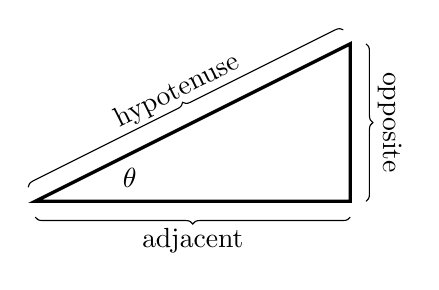
\begin{tikzpicture}
    \coordinate (C) at (0,2);
    \coordinate (D) at (4,2);
    \coordinate (E) at (4,4);
    \tkzMarkRightAngle(C,D,E)
    \tkzMarkAngle(D,C,E)
    \draw[decoration={brace,mirror,raise=.2cm},decorate,thin] (0,2)--(4,2);
    \draw[decoration={brace,mirror,raise=.2cm},decorate,thin] (4,2)--(4,4);
    \draw[decoration={brace,raise=.2cm},decorate,thin] (0,2)--(4,4);
    \draw[very thick] (D)--(E)--(C)--cycle;
    \node at (2,2-.5) {adjacent};
    \node[rotate=-90] at (4+.5,3) {opposite};
    \node[rotate=26.5] at (2-.2,3+.4) {hypotenuse};
    \node at (1.2,2.3) {$\theta$};
  \end{tikzpicture}
\end{image}
we define
\[
\cos(\theta) =
\frac{\text{adjacent}}{\text{hypotenuse}}\qquad\text{and}\qquad\sin(\theta)
= \frac{\text{opposite}}{\text{hypotenuse}}.
\]
Note that when the hypotenuse is $1$, the top right corner of this triangle is the $(\cos(\theta),\sin(\theta))$ point and thus these new definitions agree with our original ones (illustrated below). In this context though, the values of sine and cosine do not depend on the scale of the
triangle so the hypotenuse need not be $1$. %If we scale a triangle by a scalefactor $k$,

%\begin{image}[2in]
%      \begin{tikzpicture}
%      \coordinate (A) at (6,2);
%      \coordinate (B) at (6,5);
%      \coordinate (C) at (0,2);
%      \coordinate (D) at (4,2);
%      \coordinate (E) at (4,4);
%      \tkzMarkRightAngle(C,A,B)
%      \tkzMarkRightAngle(C,D,E)
%      \tkzMarkAngle(D,C,E)
%      
%      
%      \draw[decoration={brace,mirror,raise=.2cm},decorate,thin] (0,2)--(6,2);
%      \draw[decoration={brace,mirror,raise=.2cm},decorate,thin] (6,2)--(6,5);
%      \draw[decoration={brace,raise=.2cm},decorate,thin] (0,2)--(6,5);
%      \draw[dashed] (A)--(B)--(C)--cycle;
%      \draw[very thick] (D)--(E)--(C)--cycle;
%      \node at (3,2-.5) {\text{$k\cdot$adjacent}};
%      \node[rotate=-90] at (6+.5,3.5) {$k\cdot$opposite};
%      \node[rotate=26.5] at (3-.2,3.5+.4) {$k\cdot$hypotenuse};
%      \node at (1.2,2.3) {$\theta$};
%      \end{tikzpicture}
%\end{image}
%\[
%\cos(\theta) = \frac{k\cdot\text{adjacent}}{k\cdot\text{hypotenuse}} =\frac{\text{adjacent}}{\text{hypotenuse}}
%\]
%and
%\[
%\sin(\theta) = \frac{k\cdot\text{opposite}}{k\cdot\text{hypotenuse}} = \frac{\text{opposite}}{\text{hypotenuse}}.
%\]

%At this point we could simply assume that whenever we draw a triangle
%for computing sine and cosine, that the hypotenuse will be $1$. We can
%do this because we are simply scaling the triangle, and as we see
%above, this makes absolutely no difference when computing sine and
%cosine. Hence, when the hypotenuse is $1$, we find that a convenient
%way to think about sine and cosine is via the unit circle:
\begin{image}
\begin{tikzpicture}
	\begin{axis}[
            xmin=-1.1,xmax=1.1,ymin=-1.1,ymax=1.1,
            axis lines=center,
            width=4in,
            xtick={-1,1},
            ytick={-1,1},
            clip=false,
            unit vector ratio*=1 1 1,
            xlabel=$x$, ylabel=$y$,
            every axis y label/.style={at=(current axis.above origin),anchor=south},
            every axis x label/.style={at=(current axis.right of origin),anchor=west},
          ]        
          \addplot [dashed, smooth, domain=(0:360)] ({cos(x)},{sin(x)}); %% unit circle

          \addplot [textColor] plot coordinates {(0,0) (.766,.643)}; %% 40 degrees

          \addplot [ultra thick,penColor] plot coordinates {(.766,0) (.766,.643)}; %% 40 degrees
          \addplot [ultra thick,penColor2] plot coordinates {(0,0) (.766,0)}; %% 40 degrees
          
          %\addplot [ultra thick,penColor3] plot coordinates {(1,0) (1,.839)}; %% 40 degrees          

          \addplot [textColor,smooth, domain=(0:40)] ({.15*cos(x)},{.15*sin(x)});
          %\addplot [very thick,penColor] plot coordinates {(0,0) (.766,.643)}; %% sector
          %\addplot [very thick,penColor] plot coordinates {(0,0) (1,0)}; %% sector
          %\addplot [very thick, penColor, smooth, domain=(0:40)] ({cos(x)},{sin(x)}); %% sector
          \node at (axis cs:.15,.07) [anchor=west] {$\theta$};
          \node[penColor, rotate=-90] at (axis cs:.84,.322) {$y=\sin(\theta)=opp$};
          \node[penColor2] at (axis cs:.383,0) [anchor=north] {$x=\cos(\theta)=adj$};
          %\node[penColor3, rotate=-90] at (axis cs:1.06,.322) {$\tan(\theta)$};
        
        \end{axis}
\end{tikzpicture}
\end{image}

If we consider all possible combinations of ratios of
\begin{center}
  adjacent, \qquad opposite, \qquad hypotenuse,
\end{center}
(allowing the adjacent and opposite to be negative, as on the unit
circle) we obtain ratio definitions for all of the trigonometric functions.

\begin{definition}
  \index{sine}
  \index{cosine}
  \index{tangent}
  \index{secant}
  \index{cosecant}
  \index{cotangent}
  The trigonometric functions\index{trigonometric function} are:
  \[
  \begin{aligned}
  \cos(\theta) &= \frac{\text{adj}}{\text{hyp}}\\
  \sin(\theta) &= \frac{\text{opp}}{\text{hyp}}\\  
  \tan(\theta) &= \frac{\sin(\theta)}{\cos(\theta)}=\frac{\text{opp}}{\text{adj}}\qquad
  \end{aligned}
  \qquad
  \begin{aligned}
  \sec(\theta) &= \frac{1}{\cos(\theta)}=\frac{\text{hyp}}{\text{adj}}\\
  \csc(\theta) &= \frac{1}{\sin(\theta)}=\frac{\text{hyp}}{\text{opp}}\\
  \cot(\theta) &= \frac{\cos(\theta)}{\sin(\theta)} =\frac{\text{adj}}{\text{opp}}   
  \end{aligned}
  \]
  where the domain of sine and cosine is all real numbers, and the
  other trigonometric functions are defined precisely when their
  denominators are nonzero.
\end{definition}

\begin{question}
  Which of the following expressions are equal to $\sec(\theta)$?
  \begin{selectAll}
    \choice[correct]{$\frac{1}{\cos(\theta)}$}
    \choice{$\frac{1}{\sin(\theta)}$}
    \choice{$\frac{\text{adj}}{\text{hyp}}$}
    \choice[correct]{$\frac{\text{hyp}}{\text{adj}}$}
    \choice{$\frac{\tan(\theta)}{\sin(\theta)}$}
    \choice{$\frac{1}{\sin(\theta)\cdot\cot(\theta)}$}
  \end{selectAll}
  \begin{feedback}
    Note, $\frac{\tan(\theta)}{\sin(\theta)}\ne \sec(\theta)$, and
    $\frac{1}{\sin(\theta)\cdot\cot(\theta)}\ne \sec(\theta)$ since
    they differ when $\theta =0$.
  \end{feedback}
\end{question}

\begin{question}
Given the right triangle below, determine all six trig functions of unknown angle $\theta$.

\begin{image}
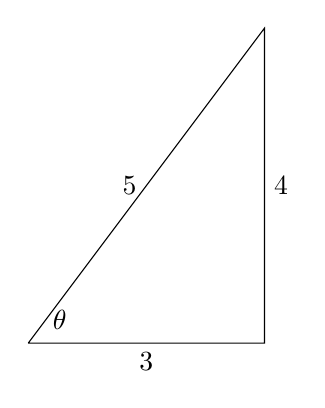
\begin{tikzpicture}
    \coordinate (C) at (0,0);
    \coordinate (D) at (3,0);
    \coordinate (E) at (3,4);
\draw (0,0) -- (3,0) node[midway,below] {$3$}
   -- (3,4) node[midway,right] {$4$}
   -- (0,0) node[midway,left] {$5$};
       \node at (0.4,0.3) {$\theta$};
       \tkzMarkRightAngle(C,D,E)
\end{tikzpicture} \end{image}
\begin{explanation}
Observe that in this triangle, adjacent=$3$, opposite=$4$, and hypotenuse=$5$. Thus without even knowing the exact value of $\theta$ we can compute:
\\$\sin(\theta)=\frac{\text{opp}}{\text{hyp}}=\frac{4}{5}$
\\$\cos(\theta)=\frac{\text{adj}}{\text{hyp}}=\frac{3}{5}$
\\$\tan(\theta)=\frac{\text{opp}}{\text{adj}}=\frac{4}{3}$
\\$\csc(\theta)=\frac{1}{\sin(\theta)}=\frac{1}{4/5}=\frac{5}{4}$
\\$\sec(\theta)=\frac{1}{\cos(\theta)}=\frac{1}{3/5}=\frac{5}{3}$
\\$\cot(\theta)=\frac{1}{\tan(\theta)}=\frac{1}{4/3}=\frac{3}{4}$
\end{explanation}
\end{question}


\subsection{Learning Objectives}
After completing this section, students should be able to:
\vspace{.05in}

\noindent$\bullet$ Draw angles given in radians or degrees in standard position, including angles that are negative or greater than a full rotation.
\\$\bullet$ Convert angles between radians and degrees using an appropriate conversion factor.
\\$\bullet$ Understand the meaning of sine and cosine as they relate to the unit circle and angles.
\\$\bullet$ Memorize the sine and cosine values of the angles in quadrant 1.
\\$\bullet$ Compute the sine or cosine of any angle that lands in one of the 16 special positions on the unit circle.
\\$\bullet$ Compute the tangent, secant, cosecant, or cotangent of any angle that lands in one of the 16 special positions on the unit circle.
\\$\bullet$ Use a given right triangle to compute trig values of an acute angle.
\\$\bullet$ Set up a right triangle with given trig value.








\end{document}